\documentclass[12pt]{report}

%language packages
\usepackage[utf8]{inputenc}
\usepackage[T1]{fontenc}
\usepackage[italian]{babel}  

%images packages
\usepackage{graphicx}
\graphicspath{ {images/} }

\usepackage{lettrine} % to get a first giant section letter
\usepackage{float} % used to float a figure (H option)
\usepackage{sidecap} % used to place a caption beside a figure

\usepackage{listings}
\lstset{
  language=bash,
  basicstyle=\ttfamily
}
\newcommand{\vitcoin}{\textit{V}itCoin}

\title{
    \Large{{UNIVERSITÀ DEGLI STUDI DI NAPOLI PARTHENOPE}}\\
    {Corso di Laurea in Informatica}\\
    {Dipartimento di Scienze e Tecnologie}\\
    \vspace{0.5cm}
    
\includegraphics[scale=0.70]{Parthenope_logo.png}\\
	{\textbf{Progetto per l'esame di \\ \textit{Reti dei Calcolatori:}}}\\
    {\textbf{\vitcoin}}
}
\author{Vittorio Zavino}
\date{\today}


\usepackage{hyperref}

\begin{document}

\maketitle

\tableofcontents
\listoffigures

\chapter{Descrizione progetto}
\section{Traccia progetto}
\lettrine{L}{a} seguente relazione è stata realizzata per descrivere il progetto realizzato per la traccia scelta: \textit{BitCoin}.
\\Tale traccia prevede lo sviluppo e la gestione di una criptovaluta  (come il \textit{BitCoin} appunto) mediante l'utilizzo di una blockchain. \\Tuttavia un caso reale di implementazione prevederebbe tutta una serie di concetti\footnote{concetti quali \textit{mining, cifratura, validazione blocchi, creazione di hash} ecc, sono stati evitati o comunque implementati in maniera semplificata(simbolica). Tutto sarà  spiegato più avanti nei rispettivi paragrafi.}, casistiche e problemi da risolvere non esplicitamente richiesti dalla traccia, la quale, per questo motivo viene riportata di seguito in modo da poter spiegare le scelte effettuate per l'implementazione.

\section*{Descrizione generale}
Si vuole realizzare un sistema per la gestione di una criptovaluta basato su una rete P2P. \\ Il sistema è basato sulla gestione di una blockchain, ovvero una sequenza di blocchi in cui ogni blocco contiene una transazione.\\
Il sistema si compone di due tipi di nodi: NodiN e NodiW. I NodiN creano la rete P2P e gestiscono la blockchain. Inoltre stampano la blockchain ogni volta che viene aggiunto un blocco: (blocco 1)->(blocco 2)->(blocco 3)->(blocco 4). \\I NodiW gestiscono i wallet (portafogli virtuali) che consentono di inviare e ricevere pagamenti. Ad ogni nuovo pagamento inviato o ricevuto il nodo stampa la transazione ed il totale del portafogli.

\subsection*{Descrizione dettagliata NodoW}
Un NodoW per ricevere un pagamento fornisce il proprio nome (IP PORTA) ed attende di ricevere il blocco contenente la transazione corrispondente. Ricevuta la transazione si somma l’ammontare al totale del wallet. \\Per effettuare un pagamento si crea una transazione formata da:\\ IP PORTA MITT:AMMONTARE:IP PORTA DEST:NUMERO RANDOM e la si invia ad un NodoN cui il NodoW è connesso.

\subsection*{Descrizione dettagliata NodoN}
Ogni NodoN gestisce una copia della blockchain, una sequenza di blocchi in cui ogni blocco contiene una transazione. \\Un blocco contiene: il numero di blocco progressivo, tempo di attesa random, transazione (IP PORTA MITT:AMMONTARE:IP PORTA DEST:NUMERO RANDOM). \\Una blockchain inizia con un blocco genesi, ovvero un blocco uguale per tutti i NodiN. Un NodoN che riceve una transazione, la memorizza in un blocco, attende un tempo random (in [5,15] sec) che inserisce nel blocco, inserisce il blocco in testa alla blockchain e lo invia a tutti i NodiN e NodiW connessi. \\Un NodoN che riceve un nuovo blocco lo inserisce in testa alla blockchain e se si trova nella fase di attesa per l’inserimento di un blocco con lo stesso numero progressivo, invalida il proprio blocco, crea un nuovo blocco e tenta nuovamente l’inserimento. \\Nel caso in cui un NodoN ricevesse un blocco con lo stesso numero progressivo del blocco in testa alla blockchain, lo inserirebbe allo stesso livello della testa (in questo modo in testa alla blockchain ci possono essere più blocchi diversi). Nel caso in cui si dovesse aggiungere un blocco ad una blockchain con più blocchi in testa, si sceglierebbe il blocco che presenta la maggiore somma dei tempi di attesa random a partire dal primo.

\textbf{Opzionale}: nel caso di aggiunta di un blocco ad una blockchain con più nodi in testa, dopo aver aggiunto il nuovo blocco dopo il blocco che presenta la maggiore somma dei tempi di attesa random a partire dal primo, rimuovere tutti gli altri blocchi dello stesso livello. Il nodo che aveva per primo aggiunto un blocco duplicato ha la responsabilità di creare un nuovo blocco e tentare nuovamente l’inserimento.

\section{Definizioni e Assunzioni}
A scanso di equivoci, verranno adesso date le seguenti \textbf{definizioni} usate nella relazione, corrispondenti ad elementi della traccia:
\begin{itemize}
\item[•] \textit{NodiN} chiamati da ora in poi \textbf{peer}.

\item[•] \textit{NodiW} chiamati da ora in poi \textbf{wallet}.

\item[•] I \textit{blocchi in testa} alla blockchain saranno chiamati \textbf{code}. Quindi in caso di inserimento di un blocco  con lo stesso numero di sequenza di una coda, si parlerà di inserimento di una \textbf{multicoda}.
\item[•] l'accoppiata \textit{IP PORTA} viene rappresentata dalla \textbf{Net\_ent}, la quale consiste in una struct contenente appositi campi \footnote{una stringa per l'indirizzo IP e un unsigned short per la porta.}.
\item[•] Il nome scelto per la criptomoneta è \textbf{\vitcoin} per ovvie ragioni.
\end{itemize}
 
Inoltre vengono qui esplicitate le seguenti \textbf{assunzioni} (spiegate nel dettaglio più avanti) fatte per semplificare la gestione della rete p2p e della blockchain:
\begin{itemize}
\item[•]\textbf{crush dei peer non gestito:} si assume che i peer che sono riusciti a connettersi alla rete non possano crushare, ma che possano soltanto essere chiusi volontariamente. Ciò viene fatto per i seguenti motivi:
\begin{itemize}
\item l'unico modo che hanno,  i peer che erano connessi al peer crushato, per "capire" se sono ancora connessi alla rete\footnote{cioè per capire se il grafo rappresentante la rete sia ancora una grafo connesso} è quello di mantenere la topologia di tutta rete appunto. Ciò permetterebbe ai suddetti peer di connettersi ai peer necessari per garantire la loro connessione diretta (o indiretta) al resto della rete\footnote{i peer a cui connettersi potrebbero essere scelti attraverso un algoritmo di costruzione di un \textit{MST: Minimum Spanning Tree}}.
\item Un altro motivo è quello della difficoltà nel sincronizzare le blockchain tra, i peer che erano stati tagliati fuori dalla rete momentanemente e quelli a cui essi si connettono per riconntersi alla rete.
\end{itemize}
\item[•]\textbf{dimensioni della rete piccola:} tale assunzione e re sa possibile ovviamente dal fatto che il progetto sia ai fini universitari. Essa viene fatta sostanzialmente per "garantire"\footnote{ovviamente data la contemporaneità  dell'attività dei peer, al crescere del numero di questi, questa "garanzia simbolica" va sempre più a diminuire} il fatto che ad un peer non arrivino mai blocchi con un numero di sequenza inferiore al numero dell' ultimo  blocco inserito nella propria blockchain.\\ Ciò significa che è possibile inserire solo blocchi con un numero di sequenza uguale (multicoda) o successivo al numero di sequenza dell'ultimo blocco appunto. A sua volta tale meccanismo semplifica l'implementazione della parte \textbf{opzionale} della traccia come spiegato più avanti nell'apposito paragrafo.
\end{itemize}



\chapter{Architettura di rete}
\lettrine{L}{a} rete è stata implementata come una rete  \textbf{\textit{p2p decentralizzata ibrida e non strutturata}}, composta da:
\begin{itemize}
\item[•] un \textbf{server} centrale, il cui unico compito è quello di tenere una lista dei peer che si sono connessi alla rete chiedendo ad esso l'autorizzazione.
\item[•] un numero dinamico di \textbf{peer}, che costituiscono la overlay network e mantengono la blockchain. 
\item[•] un numero indefinito di \textbf{wallet} che costituiscono i client dei peer e che permettono all'utente di effettuare varie transazioni di \vitcoin.
\end{itemize}

\begin{SCfigure}
  \centering
  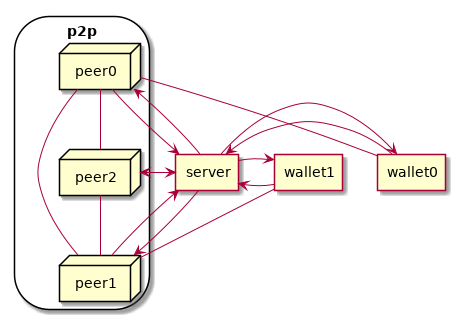
\includegraphics[scale=0.45]{arch.png}    
  \caption[architettura della rete]{\textbf{architettura della rete}: rappresentazione grafica della rete descritta sopra.\\ Le connessioni sono rappresentate dalle linee semplici, mentre le frecce rappresentano lo scambio di informazioni}
\end{SCfigure}

\section{Server}
Il server si occupa solo ed esclusivamente di dell'indirizzamento delle connessioni. Tale compito si divide sostanzialmente in 3 sottocompiti:
\begin{itemize}
\item indicare ad i nuovi peer, i peer a cui connettersi.
\item indicare ad i wallet, il peer a cui connettersi.
\item eliminare i peer che si autoterminano, dalla lista che rappresenta la rete.
\end{itemize}
 
\section{Peer}
Un peer in quanto tale, si comporta sia da \textit{client}(verso altri peer e il server) che da \textit{server} (verso altri peer e verso i wallet ad esso collegato).\\ Esso di  occupa sostanzialmente di effettuare 3 macro compiti:
\begin{itemize}
\item[•] \textit{mantenere la rete p2p}, stabilendo e gestendo le connessioni con gli altri peer.
\item[•] \textit{gestire la blockchain}, aggiornandola con i blocchi provenienti dagli altri peer e diffondendo i blocchi creati.
\item[•] \textit{soddisfare le rischieste di un wallet}, interagendo  con la blockchain leggendo o inserendo blocchi che riguardano il wallet stesso. 
\end{itemize}

\section{Wallet}
Il wallet consiste nel client messo a disposizione per gestire il proprio portafogli di \vitcoin. Esso interagendo con il peer assegnatogli dal server permette di:
\begin{itemize}
\item[•] \textit{"mining"} di nuovi \vitcoin. 
\item[•] effetuare una transazione verso un altro wallet.
\item[•] richiedere un refresh del bilancio del wallet.
\end{itemize}


\chapter{Protocollo applicazione}
\lettrine{I}{n} questo capitolo si andranno a mostrare i protocolli usati per l'implementazione delle operazioni compiute dall'entità di rete. Si farà inoltre uso di \textit{sequence diagram} per i protocolli più articolati.

\section{Protocolli Server}
Il server come descritto precedentemente si occupa di eseguire le tre operazioni descritte precedentemente per la gestione della lista dei peer. Per questo motivo esso è stato implementato come semplice server iterativo, implementazione che, unita al basso tasso di richieste da servire e al meccanismo di autorizzazione di seguito descritto, evita inutile spreco di risorse.

\subsection{Protocollo d'autenticazione}
Il protocollo d'autenticazione viene eseguito sia dai peer che dai wallet che effetuano una richiesta di aggancio alla rete al server.\\ Tale protocollo prevede l'invio della password \footnote{la password viene scelta in fase di lancio del server passandola con l'apposita opzione da riga di comando. In caso di omissione, la password di default utilizzata è "VitCoin".} di rete inviata sotto forma di hash da parte del client. Se la password è corretta, il server invierà una conferma e si metterà in attesa della macro corrispondete ad una delle operazioni che è in grado di svolgere. Altrimenti comunicherà al client che la password è sbagliata è si metterà in attesa di nuove richieste di autenticazione.

\subsection{Protocollo d'aggancio peer}
\begin{figure}[H]
  \centering
  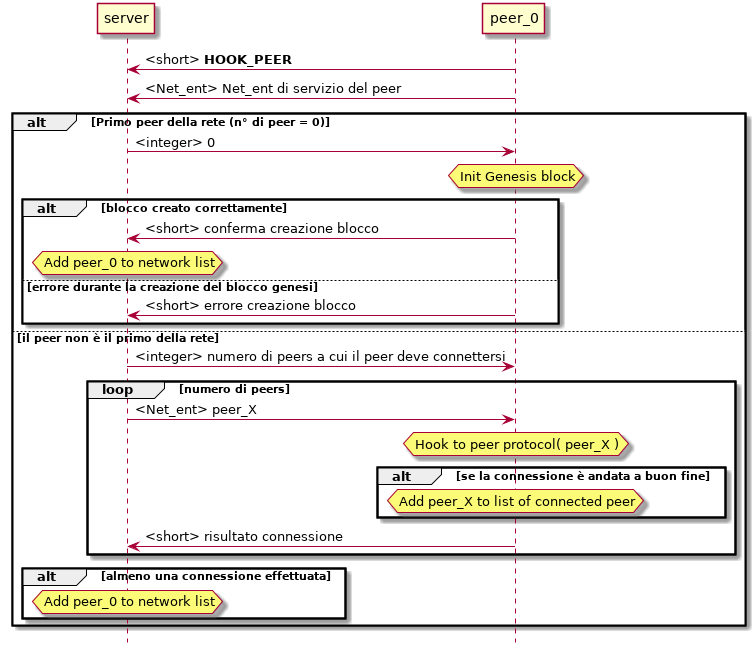
\includegraphics[scale=0.50]{hookpeer.png}    
  \caption{aggancio di un peer alla rete}
  \label{fig:hook_peer}
\end{figure}

La figura \ref{fig:hook_peer} mostra il protocollo che scatta con l'invio della apposita macro\footnote{HOOK\_PEER}, subito dopo l'autenticazione andata a buon fine da parte del peer. \\Il protocollo inizia con il peer che invia la propria Net\_ent di servizio al server. Da qui in poi le casistiche possibili sono 2:

\begin{enumerate}
\item il peer che si sta agganciando alla rete \textit{è il primo}. \\Ciò comporta che il server si mette in attesa della conferma di avvenuta crazione del blocco genesi da parte del peer. In caso di esito positivo il server lo aggiunge alla rete.
\item il peer che si sta agganciando alla rete \textit{non è il primo}. \\ In questo caso il server invia il numero minimo di peers con cui il nuovo peer deve provare la connessione. Successivamente invia uno alla volta le Net\_ent di servizio dei peer e conta il numero di connessioni riuscite al nuovo peer. Se almeno una connessione è riuscita, il nuovo peer viene aggiunto alla rete.
\end{enumerate}

\subsection{Protocollo d'aggancio wallet}
Il protocollo d'aggancio di un wallet alla rete è molto più semplice di quello utilizzato dai peer.\\ Infatti esso si compone al più di sue sole comunicazioni.
Dopo la corretta autenticazione e l'invio della macro  corrispondente da parte del wallet\footnote{HOOK\_WALLET}, il server gli invia sotto forma di intero il numero di peer attualmente presenti nella rete. Se tale numero è maggiore di 0 allora il server sceglie un peer a caso e ne invia la Net\_ent di servizio al wallet.

\subsection{Protocollo di chiusura peer}
Protocollo ancora più semplice che prevede che, un peer facente parte della rete che sta per spegnersi (dopo essersi autenticato ed aver inviato l'apposita macro\footnote{CLOSE\_PEER}) invii la propria Net\_ent di servizio al server, il quale la estrarrà dalla lista di Net\_ent rappresentante la rete.

\section{Protocolli Peer}
Come detto precedentemente un peer si occupa sostanzialmente di 3 macro compiti riguardanti rispettivamente: la gestione delle connessioni con gli altri peer e i wallet; l'aggiornamento della sua copia della blockchain con diffusione dei blocchi creati;  servire le richieste dei wallet.\\
L'aggancio alla rete del peer è stato spiegato nella parte che riguarda l'interazione con il server nella sezione precedente. 
In questa sezione saranno spiegati i protocolli che prevedono la comunicazione fra peer riguardanti la gestione delle connessioni e la trasmissione di blocchi.\\
I protocolli riguardanti le comunicazioni fra peer e wallet saranno invece spiegati nella sezione riguardante quest'ultimi.

\subsection{Protocollo d'aggancio ad un peer}
\begin{figure}[H]
  \centering
  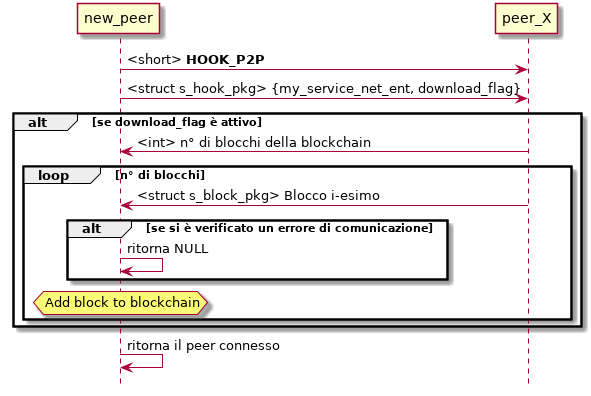
\includegraphics[scale=0.50]{hookp2p.png}    
  \caption{aggancio di un peer ad un altro peer}
  \label{fig:hook_p2p}
\end{figure}
In figura \ref{fig:hook_p2p} è mostrato il sequence diagram che spiega la funzione si permette ad un nuovo peer di agganciarsi ad un peer già agganciato alla rete. \\ Dopo l'apposita macro\footnote{HOOK\_P2P}, il nuovo peer invia un pacchetto contenente la propria Net\_ent di servizio e un flag passato come parametro, il quale indica se il nuovo blocco desidera oppure no scaricare la blockchain. \\L'utilità di tale flag sta nel fatto che un nuovo peer che si aggancia alla rete, si aggancia al numero di peer indicatogli dal server. Tuttavia risulta necessario effettuare il download della blockchain solo dal primo peer, il quale, a sua volta, (una volta che il nuovo peer avrà terminato la connessione alla rete e sarà pronto a ricevere  blocchi) provvederà a passargli i nuovi blocchi che sono stati creati mentre l'aggancio veniva ultimato.

\subsection{Protocolli di trasmissione/ricezione blocchi}
\begin{figure}[H]
  \centering
  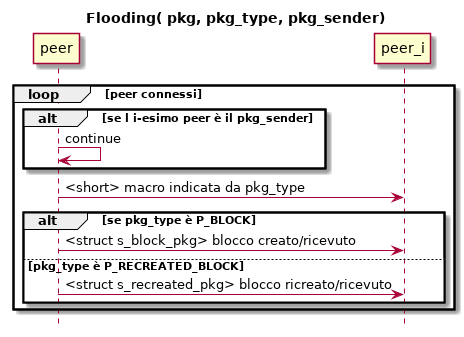
\includegraphics[scale=0.50]{flooding.png}    
  \caption{diffusione di un blocco}
  \label{fig:flooding}
\end{figure}

Come mostrato in figura \ref{fig:flooding} il protocollo di trasmissione\footnote{chiamato flooding(inondazione)  per il modo in cui viene trasmesso il blocco e cioè "inondando" i peer connessi.} è lo stesso indipendente dal tipo di blocco che si vuole trasmettere grazie all'utilizzo di un apposito flag. Viene inoltre passato come parametro la Net\_ent del peer che sta \textit{sta inviando}\footnote{il peer che \textit{invia} potrebbe essere sia il peer che sta eseguendo la funzione di flooding(cioè il creatore del blocco), sia uno dei peer connessi che ovviamente non ha bisogno di ricevere il blocco che lui stesso ci ha inviato (blocco ricevuto da altri).} il pacchetto in modo da evitare dei loop dei blocchi sulla rete.

\section{Protocolli Wallet}
In questa sezione saranno mostrati i protocolli adottati per la comunicazione del wallet con il peer a cui esso è agganciato.\\ Non si riporta la procedura d'aggancio, la quale consiste sostanzialmente solo dell'invio della apposita macro \footnote{HOOK\_W2P}, seguita dall'invio della propria Net\_ent del wallet e dalla conferma di ricezione inviata dal peer.

\subsection{Protocollo per nuova transazione}
\begin{figure}[H]
  \centering
  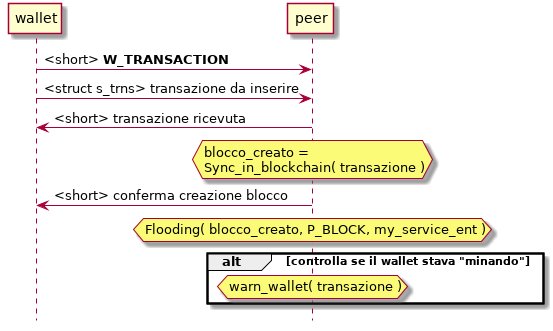
\includegraphics[scale=0.40]{w_transaction.png}    
  \caption{richiesta di una nuova transazione}
  \label{fig:w_transaction}
\end{figure}

Il protocollo utilizzato per la creazione di una nuova transazione viene usato sia nel caso di scambio di \vitcoin verso altri wallet che per il "mining"\footnote{ovviamente la procedura di mining sarà soltanto simulata, e serve sostanzialmente solo per permettere al wallet di acquisire \vitcoin come ricompensa appunto per il "mining" effettuato} di nuovi \vitcoin.

\subsection{Protocollo di richiesta saldo}
\begin{figure}[H]
  \centering
  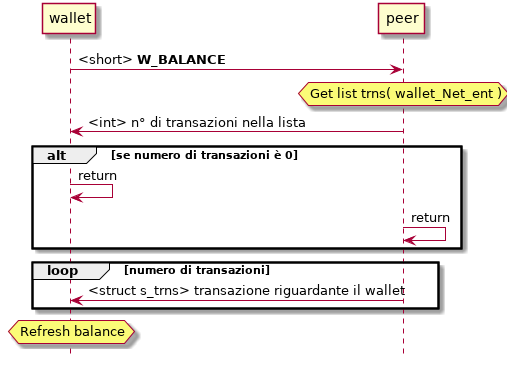
\includegraphics[scale=0.40]{w_balance.png}    
  \caption{richiesta di saldo}
  \label{fig:w_balance}
\end{figure}




\chapter{Manuale Utente}
\lettrine{L}{a} directory rilasciata contiene i seguenti elementi:
\begin{itemize}
\item[•] \textbf{CMakeLists.txt}.
\item[•] \textbf{doc/} cartella contente tutta la documentazione, copresa questa relazione.
\item[•] \textbf{LICENSE} file per il rilascio del software sotto la \textit{GNU GENERAL PUBLIC LICENSE}.
\item[•] \textbf{src/} cartella contenente tutti i sorgenti.
\end{itemize}

\subsection{Requisiti di utilizzo}
Il progetto è stato sviluppato e testato per l'utilizzo su piattaforme \textbf{Unix-like} che soddisfano i seguenti requisiti:

\begin{itemize}
\item[•]l'utility \textbf{Cmake}\footnote{\url{https://cmake.org}} versione minima 3.10.2
\item[•]la libreria \textbf{OpenSSL}\footnote{\url{https://www.openssl.org/}}
\end{itemize}

\subsection{Istruzioni per la compilazione}
Partendo dalla directory principale del progetto basterà compilare il CMakeLists.txt file, con CMake in un'apposita cartella da creare in cui poi spostarsi:

\begin{lstlisting}
$ mkdir build && cd build
\end{lstlisting}

Lanciare CMake con il comando:
\begin{lstlisting}
$ cmake ..
\end{lstlisting}

Lanciare quindi lanciare make:

\begin{lstlisting}
$ make
\end{lstlisting}

A questo punto nella directory bin (creata appositamente da cmake )saranno presenti i file eseguibili.

\subsection{Istruzioni per l'esecuzione}
\begin{lstlisting}
$ ./eseguibile -h
\end{lstlisting}

Per tutti e 3 gli eseguibili è disponibile lo \textit{Usage} mostrato a display attraverso l'opzione \textbf{-h}, il quale mostrerà tutte le possibili opzioni usabili per settare vari parametri quali ad esempio la \textit{password} da usare per l'accesso alla rete, \textit{l'indirizzo ip} e \textit{la porta del server centrale}. \\

Tutte le opzioni in quanto tali possono essere omesse abilitando i parametri di default. Tuttavia per i peer è obbligatorio fornire la \textit{port di servizio}\footnote{porta su cui il peer si mette in ascolto per le sue funzionalità da server} attraverso l'opzione \textbf{\-s}.\\

Si sottolinea infine, che attraverso l'opzione \textbf{-t}, è possibile abilitare (oltre ad un tempo non d'attesa per la creazione di un blocco non randomico), per il peer che viene lanciato per primo, la possibilità di generare oltre che al blocco genesi, anche una blockchain di prova appositamente creata per dimostrare il funzionamento della parte opzionale del progetto. Tale blockchain contiene 5 blocchi e ha come ultimo numero di sequenza 3 in modo da avere due \textbf{code}. Di conseguenza il primo nuovo blocco inserito creato farà scattare la procedura di ricreazione della coda minore in termini di tempo d'attesa. \\

Di seguito la sequenza di comandi da lanciare per un test con le opzioni di default e la fake blockchain:\\

Lancio del server
\begin{lstlisting}
$ ./server
\end{lstlisting}

Lancio di uno o più peer (numero di porta diverso per ognuno)
\begin{lstlisting}
$ ./peer -s 2222 -t 2
\end{lstlisting}

Lancio di uno o più wallet
\begin{lstlisting}
$ ./wallet
\end{lstlisting}





\end{document}


